\chapter{Implementazioni in LiSA}\label{chapter:lisa}



LiSA (\textbf{Li}brary for \textbf{S}tatic \textbf{A}nalysis) è un framework generico sviluppato come libreria open-source in Java che permette in modo facile, diretto e completo l'analisi statica tramite interpretazione astratta di semplici programmi multi linguaggio. Una basilare rappresentazione del flow dell'analisi in LiSA può essere vista in figura \ref{fig:lisaAnalysisFlow} e lo possiamo riassumere così: (1) un programma scritto in un linguaggio L viene passato al front-end appropriato che lo trascrive nel linguaggio intermedio compreso da LiSA basato su Control Flow Graph (LiSA CFG), (2) LiSA poi analizza i CFGs creati con un algoritmo di ricerca del fix-point seguendo le linee guida passate da utente tramite la configurazione (ad esempio: domini da usare, parametri per l'algorito del fix-point, tipo di analisi interprocedurale), (3) infine LiSA esegue i semantics checks, anch'essi passati da utente, ed eventualmente genera warnings ed errori se l'analisi non ne rispetta i vincoli. 

LiSA mette a disposizione: (i) un linguaggio interno basato su control-flow graph estensibile e abbastanza generico da supportare i costrutti semantici di molti linguaggi di programmazione, (ii) una vasta gamma di front-end per la traduzione di programmi in LiSA CFGs, (iii) una base comune per lo sviluppo di nuovi domini astratti da usare nelle analisi (sia relazionali che non, più alcuni domini built-in) ed infine (iv) un algoritmo per il calcolo del fix-point dei LiSA CFGs con metodo di risoluzione basato su working-set list.

Durante la mia tesi ho lavorato soprattutto sulle componenti (iii) e (iv). Per prima cosa ho esteso l'algoritmo per il calcolo del fix-point affinchè fosse in grado di eseguire anche la fase discendente partendo da un post-fix-point precedentemente calcolato, ho aggiunto classi generiche come base per l'implementazione del dominio astratto degli insiemi non ridondanti di un altro dominio astratto (nonchè una implementazione concreta di ciò per gli intervalli) ed infine, per scopo sperimentale, una rudimentale versione del decoupling capace di usare domini diversi per salire e scendere nell'analisi.

\section{LiSA}
In questa sezione faremo una overview della archutettura di LiSA facalizzandoci sulla struttura della rappresentazione interna dei programmi, sulle interfacce attraverso cui è possibile definire nuovi domini astratti e sull'organizzazione della vera e propria analisi statica (andando a guardarne le componenti e gli algoritmi).

\subsection{I CFG di LiSA}
La struttura dei CFG in LiSA è progettata per essere il più flessibile possibile così da essere in grado di rappresentare il maggior numero di costrutti semantici provenienti da più linguaggi di programmazione. Un LiSA CFG ha gli \texttt{Statement} come nodi (ognuno con il proprio significato semantico) e gli \texttt{Edge} come archi (i quali modellano il flusso di dati durante l'esecuzione del programma). 

\subsubsection{Statement}
Uno \texttt{Statement} rappresenta un costrutto semantico base di un linguaggio di programmazione che non modifica il flusso di esecuzione.  

\begin{figure}
    \centering

\tikzset{every picture/.style={line width=0.75pt}} %set default line width to 0.75pt        

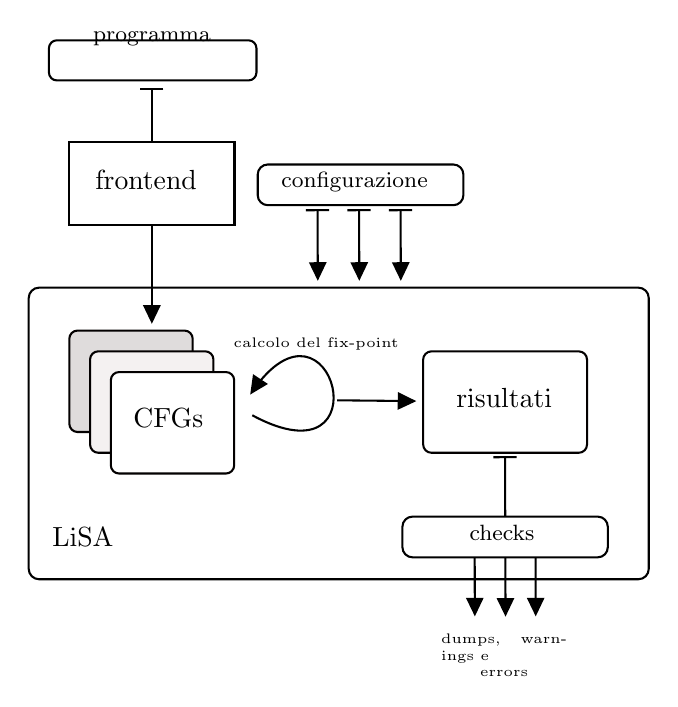
\begin{tikzpicture}[x=0.75pt,y=0.75pt,yscale=-1,xscale=1]
%uncomment if require: \path (0,373); %set diagram left start at 0, and has height of 373

%Shape: Rectangle [id:dp735576293814507] 
\draw  [fill={rgb, 255:red, 255; green, 255; blue, 255 }  ,fill opacity=1 ] (10.44,145) .. controls (10.44,142.24) and (12.68,140) .. (15.44,140) -- (304.17,140) .. controls (306.93,140) and (309.17,142.24) .. (309.17,145) -- (309.17,275.5) .. controls (309.17,278.26) and (306.93,280.5) .. (304.17,280.5) -- (15.44,280.5) .. controls (12.68,280.5) and (10.44,278.26) .. (10.44,275.5) -- cycle ;
%Straight Lines [id:da23563586478588427] 
\draw    (69.77,44.13) -- (69.77,154.4) ;
\draw [shift={(69.77,157.4)}, rotate = 270] [fill={rgb, 255:red, 0; green, 0; blue, 0 }  ][line width=0.08]  [draw opacity=0] (8.93,-4.29) -- (0,0) -- (8.93,4.29) -- cycle    ;
\draw [shift={(69.77,44.13)}, rotate = 270] [color={rgb, 255:red, 0; green, 0; blue, 0 }  ][line width=0.75]    (0,5.59) -- (0,-5.59)   ;
%Shape: Rectangle [id:dp6301022803478207] 
\draw  [fill={rgb, 255:red, 255; green, 255; blue, 255 }, fill opacity=1 ] (30,70) -- (109.57,70) -- (109.57,110) -- (30,110) -- cycle ;
%Rounded Rect [id:dp2844998293479686] 
\draw  [fill={rgb, 255:red, 255; green, 255; blue, 255 }  ,fill opacity=1 ] (20.17,24.7) .. controls (20.17,22.56) and (21.9,20.83) .. (24.03,20.83) -- (116.3,20.83) .. controls (118.44,20.83) and (120.17,22.56) .. (120.17,24.7) -- (120.17,36.3) .. controls (120.17,38.44) and (118.44,40.17) .. (116.3,40.17) -- (24.03,40.17) .. controls (21.9,40.17) and (20.17,38.44) .. (20.17,36.3) -- cycle ;
%Rounded Rect [id:dp015147798185889627] 
\draw   (120.78,85.5) .. controls (120.78,82.83) and (122.94,80.67) .. (125.61,80.67) -- (215.03,80.67) .. controls (217.7,80.67) and (219.87,82.83) .. (219.87,85.5) -- (219.87,95.43) .. controls (219.87,98.1) and (217.7,100.27) .. (215.03,100.27) -- (125.61,100.27) .. controls (122.94,100.27) and (120.78,98.1) .. (120.78,95.43) -- cycle ;
%Shape: Rectangle [id:dp3167426310658905] 
\draw  [color={rgb, 255:red, 3; green, 0; blue, 0 }  ,draw opacity=1 ][fill={rgb, 255:red, 223; green, 220; blue, 220 }  ,fill opacity=1 ] (30,164.67) .. controls (30,162.46) and (31.79,160.67) .. (34,160.67) -- (85.44,160.67) .. controls (87.65,160.67) and (89.44,162.46) .. (89.44,164.67) -- (89.44,205.56) .. controls (89.44,207.76) and (87.65,209.56) .. (85.44,209.56) -- (34,209.56) .. controls (31.79,209.56) and (30,207.76) .. (30,205.56) -- cycle ;
%Shape: Rectangle [id:dp5390943849837029] 
\draw  [color={rgb, 255:red, 3; green, 0; blue, 0 }  ,draw opacity=1 ][fill={rgb, 255:red, 255; green, 255; blue, 255 }  ,fill opacity=1 ] (200.48,174.7) .. controls (200.48,172.49) and (202.27,170.7) .. (204.48,170.7) -- (275.44,170.7) .. controls (277.65,170.7) and (279.44,172.49) .. (279.44,174.7) -- (279.44,215.56) .. controls (279.44,217.76) and (277.65,219.56) .. (275.44,219.56) -- (204.48,219.56) .. controls (202.27,219.56) and (200.48,217.76) .. (200.48,215.56) -- cycle ;
%Shape: Rectangle [id:dp6482074079685427] 
\draw  [color={rgb, 255:red, 3; green, 0; blue, 0 }  ,draw opacity=1 ][fill={rgb, 255:red, 244; green, 241; blue, 241 }  ,fill opacity=1 ] (40,174.67) .. controls (40,172.46) and (41.79,170.67) .. (44,170.67) -- (95.44,170.67) .. controls (97.65,170.67) and (99.44,172.46) .. (99.44,174.67) -- (99.44,215.56) .. controls (99.44,217.76) and (97.65,219.56) .. (95.44,219.56) -- (44,219.56) .. controls (41.79,219.56) and (40,217.76) .. (40,215.56) -- cycle ;
%Shape: Rectangle [id:dp5665391899993595] 
\draw  [color={rgb, 255:red, 3; green, 0; blue, 0 }  ,draw opacity=1 ][fill={rgb, 255:red, 255; green, 255; blue, 255 }  ,fill opacity=1 ] (50,184.67) .. controls (50,182.46) and (51.79,180.67) .. (54,180.67) -- (105.44,180.67) .. controls (107.65,180.67) and (109.44,182.46) .. (109.44,184.67) -- (109.44,225.56) .. controls (109.44,227.76) and (107.65,229.56) .. (105.44,229.56) -- (54,229.56) .. controls (51.79,229.56) and (50,227.76) .. (50,225.56) -- cycle ;
%Straight Lines [id:da034591409315066324] 
\draw [line width=0.75]    (149.61,102.69) -- (149.71,133.69) ;
\draw [shift={(149.72,136.69)}, rotate = 269.81] [fill={rgb, 255:red, 0; green, 0; blue, 0 }  ][line width=0.08]  [draw opacity=0] (8.93,-4.29) -- (0,0) -- (8.93,4.29) -- cycle    ;
\draw [shift={(149.61,102.69)}, rotate = 269.81] [color={rgb, 255:red, 0; green, 0; blue, 0 }  ][line width=0.75]    (0,5.59) -- (0,-5.59)   ;
%Straight Lines [id:da8442899163237636] 
\draw [line width=0.75]    (169.61,102.69) -- (169.71,133.69) ;
\draw [shift={(169.72,136.69)}, rotate = 269.81] [fill={rgb, 255:red, 0; green, 0; blue, 0 }  ][line width=0.08]  [draw opacity=0] (8.93,-4.29) -- (0,0) -- (8.93,4.29) -- cycle    ;
\draw [shift={(169.61,102.69)}, rotate = 269.81] [color={rgb, 255:red, 0; green, 0; blue, 0 }  ][line width=0.75]    (0,5.59) -- (0,-5.59)   ;
%Straight Lines [id:da1808180600514191] 
\draw [line width=0.75]    (189.61,102.69) -- (189.71,133.69) ;
\draw [shift={(189.72,136.69)}, rotate = 269.81] [fill={rgb, 255:red, 0; green, 0; blue, 0 }  ][line width=0.08]  [draw opacity=0] (8.93,-4.29) -- (0,0) -- (8.93,4.29) -- cycle    ;
\draw [shift={(189.61,102.69)}, rotate = 269.81] [color={rgb, 255:red, 0; green, 0; blue, 0 }  ][line width=0.75]    (0,5.59) -- (0,-5.59)   ;
%Curve Lines [id:da7168976803847669] 
\draw    (118.17,201.5) .. controls (182.52,236.15) and (156.7,134.57) .. (118.33,189.78) ;
\draw [shift={(117.17,191.5)}, rotate = 303.47] [fill={rgb, 255:red, 0; green, 0; blue, 0 }  ][line width=0.08]  [draw opacity=0] (8.93,-4.29) -- (0,0) -- (8.93,4.29) -- cycle    ;
%Straight Lines [id:da3343995640969275] 
\draw [line width=0.75]    (159,194.28) -- (194.17,194.64) ;
\draw [shift={(197.17,194.67)}, rotate = 180.58] [fill={rgb, 255:red, 0; green, 0; blue, 0 }  ][line width=0.08]  [draw opacity=0] (8.93,-4.29) -- (0,0) -- (8.93,4.29) -- cycle    ;
%Straight Lines [id:da6598443106986112] 
\draw [line width=0.75]    (239.94,221.69) -- (240.16,295.5) ;
\draw [shift={(240.17,298.5)}, rotate = 269.83] [fill={rgb, 255:red, 0; green, 0; blue, 0 }  ][line width=0.08]  [draw opacity=0] (8.93,-4.29) -- (0,0) -- (8.93,4.29) -- cycle    ;
\draw [shift={(239.94,221.69)}, rotate = 269.83] [color={rgb, 255:red, 0; green, 0; blue, 0 }  ][line width=0.75]    (0,5.59) -- (0,-5.59)   ;
%Rounded Rect [id:dp7910872057944298] 
\draw  [fill={rgb, 255:red, 255; green, 255; blue, 255 }  ,fill opacity=1 ] (190.5,255.17) .. controls (190.5,252.5) and (192.66,250.33) .. (195.33,250.33) -- (284.61,250.33) .. controls (287.28,250.33) and (289.44,252.5) .. (289.44,255.17) -- (289.44,265.1) .. controls (289.44,267.77) and (287.28,269.93) .. (284.61,269.93) -- (195.33,269.93) .. controls (192.66,269.93) and (190.5,267.77) .. (190.5,265.1) -- cycle ;
%Straight Lines [id:da7891879484603097] 
\draw [line width=0.75]    (254.64,270.28) -- (254.71,295.36) ;
\draw [shift={(254.72,298.36)}, rotate = 269.83] [fill={rgb, 255:red, 0; green, 0; blue, 0 }  ][line width=0.08]  [draw opacity=0] (8.93,-4.29) -- (0,0) -- (8.93,4.29) -- cycle    ;
%Straight Lines [id:da9550393969063078] 
\draw [line width=0.75]    (225.31,270.28) -- (225.38,295.36) ;
\draw [shift={(225.39,298.36)}, rotate = 269.83] [fill={rgb, 255:red, 0; green, 0; blue, 0 }  ][line width=0.08]  [draw opacity=0] (8.93,-4.29) -- (0,0) -- (8.93,4.29) -- cycle    ;

% Text Node
\draw (59.33,197) node [anchor=north west][inner sep=0.75pt]   [align=left] {CFGs};
% Text Node
\draw (130.67,82.75) node [anchor=north west][inner sep=0.75pt]   [align=left] {{\footnotesize configurazione}};
% Text Node
\draw (38.67,15.25) node [anchor=north west][inner sep=0.75pt]  [font=\footnotesize] [align=left] {\begin{minipage}[lt]{44.44pt}\setlength\topsep{0pt}
\begin{center}
programma
\end{center}

\end{minipage}};
% Text Node
\draw (41,82) node [anchor=north west][inner sep=0.75pt]   [align=left] {frontend};
% Text Node
\draw (20.33,254) node [anchor=north west][inner sep=0.75pt]   [align=left] {LiSA};
% Text Node
\draw (107.67,162.75) node [anchor=north west][inner sep=0.75pt]  [font=\tiny] [align=left] {calcolo del fix-point};
% Text Node
\draw (215,187) node [anchor=north west][inner sep=0.75pt]   [align=left] {risultati};
% Text Node
\draw (221.33,253.08) node [anchor=north west][inner sep=0.75pt]   [align=left] {{\footnotesize checks}};
% Text Node
\draw (207.67,305.42) node [anchor=north west][inner sep=0.75pt]  [font=\tiny] [align=left] {\begin{minipage}[lt]{45.52pt}\setlength\topsep{0pt}
dumps, warnings e
\begin{center}
errors
\end{center}

\end{minipage}};


\end{tikzpicture}
    \caption{Caption}
    \label{fig:lisaAnalysisFlow}
\end{figure}

